\section{Criterion-Level Inference and Decoding}
\subsection{Structured prediction and evidence}
The instruction prompt requests one JSON object. The parser validates the label against the criterion type, removes and records out-of-range sentence IDs, and invokes constrained label scoring if generation cannot be parsed. A decisive prediction without evidence is marked unsupported. A grounded template explains the output using only cited sentences; the aggregation rule treats unsupported or unknown criteria as requiring review rather than as a pass.

\subsection{KV-cached autoregressive decoding}
The reference decoder recomputes the full prefix. The cached decoder prefills a Hugging Face dynamic cache once, then forwards one token per step with the absolute position and an expanded attention mask. With $L$ layers, $H_{kv}$ key/value heads, head dimension $d_h$, sequence length $S$, batch $B$, and $b$ bytes per element, the cache allocation is
\begin{equation}
M_{KV}=2L B H_{kv} S d_h b.
\end{equation}
The factor two accounts for keys and values. Tests check token equality on tiny models, cache growth, byte counts, and a negative position-reset case. Timing and allocation are measured separately from correctness.
Figure~\ref{fig:kv-flow} shows that the cache is extended with each token and reused by the next decode step.

\begin{figure*}[t]
\centering
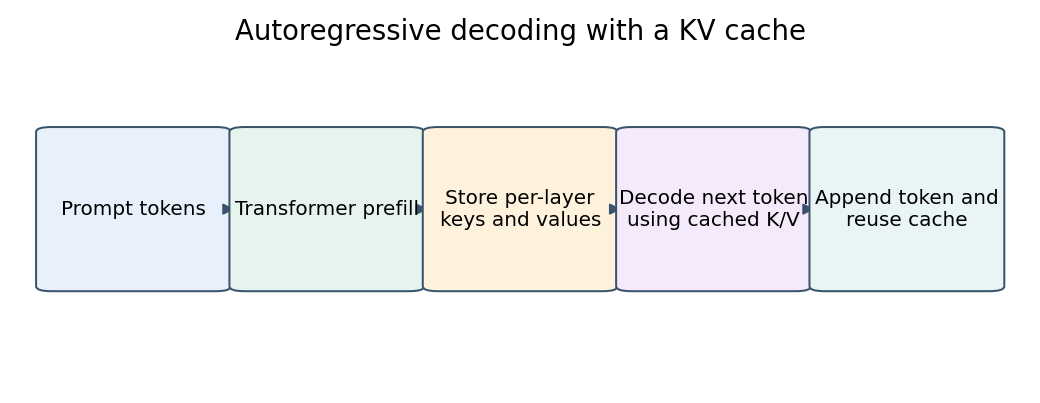
\includegraphics[width=\textwidth]{kv_cache_flow.png}
\caption{KV-cached autoregressive decoding: the prefix is prefetched once and each generated token extends the per-layer key/value cache.}
\label{fig:kv-flow}
\end{figure*}

\subsection{Tiled online-softmax attention}
The tiled implementation traverses query and key blocks and maintains a running row maximum $m$, normalizer $\ell$, and weighted-value accumulator $a$. When a new key tile changes the maximum from $m$ to $m'$, prior accumulators are rescaled by $\alpha=\exp(m-m')$, and the tile contributes its own normalized weights. The final output is $a/\ell$. This avoids storing the full score matrix while keeping accumulation in higher precision. Numerical error is compared with a double-precision reference; fused SDPA methods are performance baselines, not the implementation under test.
Figure~\ref{fig:tiled-flow} illustrates the online rescaling that permits blockwise accumulation without materializing the full score matrix.

\begin{figure*}[t]
\centering
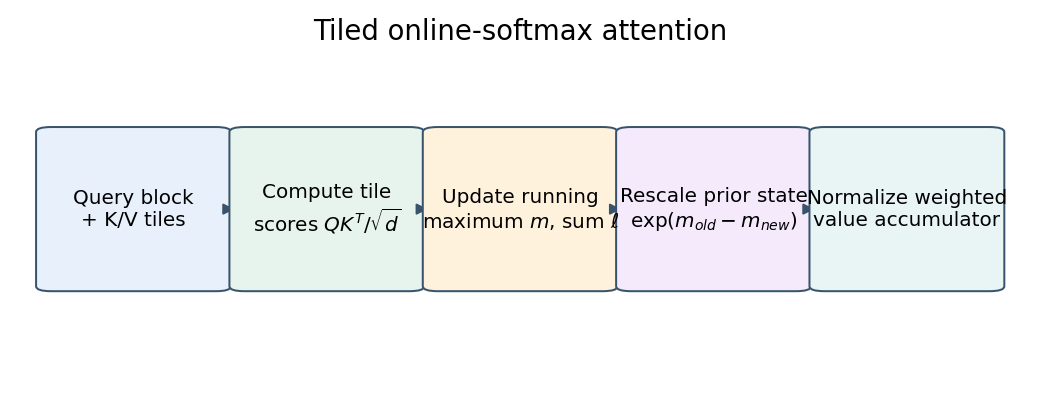
\includegraphics[width=\textwidth]{tiled_attention_flow.png}
\caption{Tiled attention maintains an online softmax state and rescales it when the running maximum changes.}
\label{fig:tiled-flow}
\end{figure*}

\subsection{Greedy speculative decoding}
The smaller model proposes up to $k$ tokens, then the target verifies the proposed block. Matching target argmax tokens are accepted; at the first mismatch the target token is emitted and the draft cache is cropped to the accepted prefix. The method is greedy and is checked for exact output equality against target KV-cache decoding. Acceptance rate and timing are reported independently because matching tokens need not yield a speedup on every hardware configuration.
Figure~\ref{fig:speculative-flow} depicts the accepted-prefix and target-correction steps for greedy decoding.

\begin{figure*}[t]
\centering
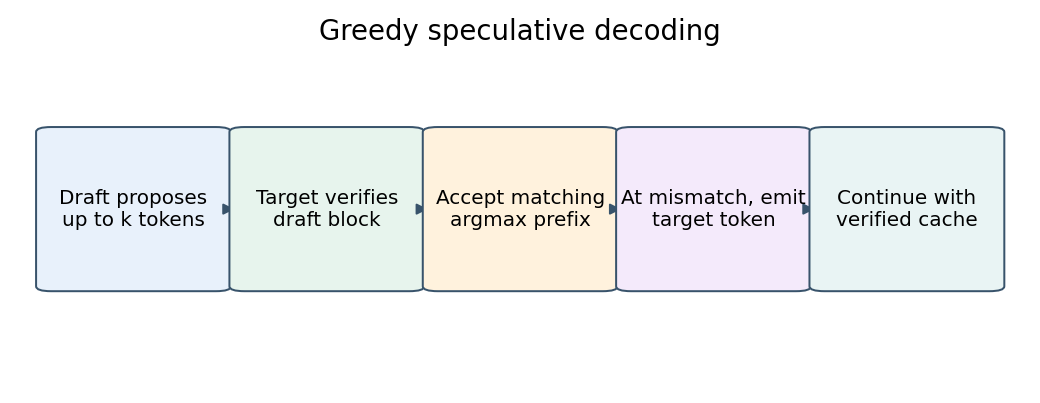
\includegraphics[width=\textwidth]{speculative_decoding_flow.png}
\caption{Greedy speculative decoding proposes a block, accepts the matching prefix, and uses the target token at the first mismatch.}
\label{fig:speculative-flow}
\end{figure*}
